%\documentclass[handout]{beamer} %Makes Handouts
\usetheme{Singapore} %Gray with fade at top
\useoutertheme[subsection=false]{miniframes} %Supppress subsection in header
\useinnertheme{rectangles} %Itemize/Enumerate boxes
\usecolortheme{seagull} %Color theme
\usecolortheme{rose} %Inner color theme

\definecolor{light-gray}{gray}{0.75}
\definecolor{dark-gray}{gray}{0.55}
\setbeamercolor{item}{fg=light-gray}
\setbeamercolor{enumerate item}{fg=dark-gray}

\setbeamertemplate{navigation symbols}{}
\setbeamertemplate{mini frames}[default]
\setbeamercovered{dynamics}
\setbeamerfont*{title}{size=\Large,series=\bfseries}

%\setbeameroption{notes on second screen} %Dual-Screen Notes
%\setbeameroption{show only notes} %Notes Output

\newcommand{\heading}[1]{\noindent \textbf{#1}\\ \vspace{1em}}

\usepackage{bbding,color,multirow,times,ccaption,tabularx,graphicx,verbatim,booktabs,fixltx2e}
\usepackage{colortbl} %Table overlays
\usepackage[english]{babel}
\usepackage[latin1]{inputenc}
\usepackage[T1]{fontenc}

%\author[]{Thomas J. Leeper}
\institute[]{
  \inst{}%
  Department of Political Science and Government\\Aarhus University
}

\usepackage{tikz}
\usetikzlibrary{shapes,arrows,decorations}

\title{Methods Supplementary Lecture 3:\\Experimentation}

\date[]{}

\begin{document}

\frame{\titlepage}

\frame{\tableofcontents}

\section{Causal Inference}
\frame{\tableofcontents[currentsection]}

\frame{
\frametitle{Physical causality}

\begin{itemize}\itemsep1em
\item Action and reaction
\item Features: Observable and deterministic
\item Example:
	\begin{itemize}
	\item Picture a ball resting on top of a hill
	\item What happens if I push the ball?
	\end{itemize}
\item Physical causality is easy to see
\end{itemize}
}

\frame{
\frametitle{Correlation I}
\begin{itemize}\itemsep1em
\item Correlation is the non-independence of two variables for a set of observations
\end{itemize}
}

\frame{
\frametitle{Correlation II}
\begin{itemize}
\item \textit{Observation}: A case or unit (e.g., person, country)
\item \textit{Variable}: A dimension that describes an obseration (e.g., income)
\item \textit{Independence}: Variables are unrelated to one another
	\begin{itemize}
	\item Independent: Height and value on a fair dice roll
	\item Non-independent: Height and weight
	\end{itemize}
\end{itemize}
}


\frame{
\frametitle{Correlation III}

\begin{itemize}\itemsep1em
\item Synonyms: correlation, covariation, relationship, association
	\begin{itemize}
	\item ``Effect'' is frequently used to mean correlation
	\item We'll reserve that term for a \textit{causal effect}
	\end{itemize}
\item Any correlation is a potential cause
	\begin{itemize}
	\item X might cause Y
	\item Y might cause X
	\item X and Y might be caused by Z
	\item X and Y might cause Z
	\item There may be no causal relationship
	\end{itemize}
\end{itemize}
}

\frame<1>[label=mill]{

\frametitle{Mill's methods\footnote{Discussed in Holland}}

\begin{itemize}
\item Agreement
\item \textbf<2>{Difference}
\item Agreement and Difference
\item Residue
\item Concomitant variations
\end{itemize}
}

\frame{
\frametitle{Difference}

If an instance in which the phenomenon under investigation occurs, and an instance in which it does not occur, have every circumstance save one in common, that one occurring only in the former; the circumstance in which alone the two instances differ, is the effect, or cause, or an necessary part of the cause, of the phenomenon.
}

\frame{

\frametitle{Four (or five) principles of causality\footnote{From Kellstedt and Whitten}}

\begin{enumerate}
\item Correlation
\item Nonconfounding
\item Direction (``temporal precedence'')
\item Mechanism
\item (Appropriate level of analysis)
\end{enumerate}
}


\frame{\huge\vskip20pt\textbf{Questions?}}



\frame[label=counterfactuals]{
\frametitle{Counterfactual Thinking}

\begin{itemize}\itemsep1em
\item \textit{Counterfactual}: relating to what has not happened or is not the case
\vspace{0.5em}
\item Causal inference involves inferring \textit{what would have happened} in a counterfactual reality \textit{where the potential cause took on a different value}
\end{itemize}

}

% Has anyone read or seen *A Christmas Carol*?

\frame{
\frametitle{``A Christmas Carol''}

\small 
\begin{itemize}
\item 1843 novel by Charles Dickens
\item Ebenezer Scrooge is shown his own future by the ``Ghost of Christmas Yet to Come''
\item Has the choice to either:
	\begin{itemize}
	\item stay on current path (one counterfactual), or 
	\item change his ways (take a different counterfactual)
	\end{itemize}
\end{itemize}
}

\frame{
\frametitle{Causation}

\begin{itemize}\itemsep1em
\item \textit{Causal effect}: The difference between two ``potential outcomes''
	\begin{itemize}
	\item The outcome that occurs if $X = x_1$
	\item The outcome that occurs if $X = x_2$
	\end{itemize}
\item The causal effect of Scrooge's lifestyle is seen in the differences between two potential futures
\end{itemize}

}

\frame{
\frametitle{Fundamental problem of causal inference}

\Large We can only observe any given unit in one reality!

}

\frame{
\frametitle{Two solutions!\footnote{From Holland}}

\begin{enumerate}\itemsep1em
\item Scientific Solution
	\begin{itemize}
	\item All units are identical
	\item Each can provide a perfect counterfactual
	\item Common in, e.g., agriculture, biology
	\end{itemize}
\item<2-> Statistical Solution
	\begin{itemize}
	\item Units are not identical
	\item Random exposure to a potential cause
	\item Effects measured on average across units
	\item Known as the ``Experimental ideal''
	\end{itemize}
\end{enumerate}

}

\frame{
\frametitle{In Political Science}

\small

\begin{itemize}\itemsep0.5em
\item Causal inference is about searching for appropriate counterfactuals
	\begin{itemize}
	\item<2-> \textit{Causal effect}: Difference in an outcome variable between two counterfactuals
	\item<3-> \textit{Causal inference}: A belief that an event or variable exerts a causal effect on an outcome
	\end{itemize}
\item<4-> Where can we look for counterfactuals?
\end{itemize}

}

\frame{

\frametitle{An Example}

\small

\begin{itemize}\itemsep0.5em
\item For example, if we think smoking might cause lung cancer, how would we know?
\vspace{0.5em}
\item How would we know if smoking caused lung cancer for an individual who smoked?
	\begin{itemize}
	\item What's the relevant counterfactual?
	\end{itemize}
\item How would we know if smoking causes lung cancer on average across many individuals?
	\begin{itemize}
	\item What's the relevant counterfactual?
	\end{itemize}
\end{itemize}

}


\section{Randomization}
\frame{\tableofcontents[currentsection]}

\frame{
	\frametitle{Observational Causal Inference}
	\begin{itemize}\itemsep2em
		\item Find all variables Z
		\item Control for influence of Z to identify effect of $X \rightarrow Y$
		\item<2-> One common strategy is \textit{matched sampling} or \textit{matching}
		\item<3-> Regression is similar, but we'll talk about that later
	\end{itemize}
}

\frame{
	\frametitle{Matching I}
	\begin{itemize}\itemsep2em
    	\item Example: Effect of Education on Participation
    	\item Our design involves:
    		\begin{itemize}
    		\item Measure outcome (participation)
    		\item Measure putative cause (education; university degree)
    		\item Correlate outcome and cause
    		\end{itemize}
    	\item Is that correlation a valid causal inference?
	\end{itemize}
}

\frame{
	\frametitle{Matching II}
	\begin{itemize}\itemsep2em
    	\item Temporal ordering is correct here
    		\begin{itemize}
    		\item Note: Timing of measurement may be unimportant
    		\end{itemize}
    	\item<2-> What about confounding?
    		\begin{enumerate}
    		\item<3-> Hide outcome data
    		\item<4-> List all potential confounds (Z)
    		\item<5-> Match observations so sample consists of pairs of observations (1 with degree; 1 without) that are identical (or at least similar) on all variables
    		\item<6-> Discard all observations that cannot be matched
    		\item<7-> Estimate $Corr(X,Y)$
    		\end{enumerate}
	\end{itemize}
}

\frame{
	\frametitle{Think--Pair--Share}
	\begin{itemize}\itemsep1em
    	\item Does matching always get us to a clear and uncontroversial causal inference?
    	\item Think for 15 seconds to yourself
    	\item Then discuss with the person sitting next to you
	\end{itemize}
}

\frame{
	\frametitle{The Experimental Ideal}
	\begin{itemize}\itemsep0.5em
    	\item Randomized experiment, or randomized control trial
    		\begin{itemize}
    			\item \textit{The observation of units after, and possibly before, a randomly assigned intervention in a controlled setting, which tests one or more precise causal expectations}
    		\end{itemize}
    	\item A correctly executed experiment always provides clear causal inference
    	\item It solves both the temporal ordering and confounding problems
    		\begin{itemize}
        		\item Treatment (X) is applied by the researcher before outcome (Y)
        		\item Randomization means there are no confounding (Z) variables
    		\end{itemize}
	\end{itemize}
}

\frame{
	\frametitle{Experiments}
	\begin{itemize}\itemsep0.5em
		\item American Political Science Association president A. Lawrence Lowell (1909):\\ \textit{``We are limited by the impossibility of experiment. Politics is an observational, not an experimental science...''}
		\item First political science experiment: Gosnell (1926)
		\item Experiments prominent in psychology and the physical sciences
		\item King, Keohane, and Verba (1994) only mentions experiments once
	\end{itemize}
}

\frame{
	\frametitle{Causal Inference in Experiments I}
	\begin{itemize}\itemsep0.5em
    	\item<1-> Causal inference is a comparison of two \textit{potential outcomes}
    	\item<2-> A potential outcome is the value of the outcome (Y) for a given unit (i) after receiving a particular version/level/amount of the treatment (X)
    	\item<3-> Each unit has multiple \textit{potential} outcomes, but we only observe one of them
    	\item<4-> A \textit{causal effect} is the difference between two potential outcomes (e.g., $Y_{X=1} - Y_{X=0}$), all else constant
	\end{itemize}
}

\frame{
	\frametitle{Causal Inference in Experiments II}
	\begin{itemize}\itemsep2em
    	\item<1-> We cannot see individual-level causal effects
    	\item<2-> We can see \textit{average causal effects}
    		\begin{itemize}
        		\item<2-> Ex.: Average difference in participation between those with and without university degrees
    		\end{itemize}
    	\item<3-> We want to know: $TE_i = Y_{1i} - Y_{0i}$
	\end{itemize}
}

\frame{
	\frametitle{Causal Inference in Experiments III}
	\begin{itemize}\itemsep1em
		\item<1-> We want to know: $TE_i = Y_{1i} - Y_{0i}$
		\item<2-> We can average: $ATE = E[Y_{1i} - Y_{0i}] = E[Y_{1i}] - E[Y_{0i}]$
		\item<3-> But we still only see one potential outcome for each unit:\\ \vspace{1em}
    		$ATE_{naive} = E[Y_{1i} | X = 1] - E[Y_{0i} | X = 0]$
    	\item<4-> Is this what we want to know?
	\end{itemize}
}


\frame{
	\frametitle{Causal Inference in Experiments IV}
	\begin{itemize}\itemsep1em
	\item What we want and what we have:
		\begin{align}
		ATE & = E[Y_{1i}] - E[Y_{0i}] \\[1em]
		ATE_{naive} & = E[Y_{1i} | X = 1] - E[Y_{0i} | X = 0]
		\end{align}		
	\item<2-> Are the following statements true?\\
  		\begin{itemize}\itemsep1em
      		\item<2-> $E[Y_{1i}] = E[Y_{1i} | X = 1]$
      		\item<2-> $E[Y_{0i}] = E[Y_{0i} | X = 0]$
  		\end{itemize}
  	\item<3-> Not in general!
  	\end{itemize}
}

\frame{
	\frametitle{Causal Inference in Experiments V}
	\begin{itemize}\itemsep1em
    	\item Only true when both of the following hold:
    	\begin{align}
    	E[Y_{1i}] = E[Y_{1i} | X = 1] = E[Y_{1i} | X = 0]\\
    	E[Y_{0i}] = E[Y_{0i} | X = 1] = E[Y_{0i} | X = 0]
    	\end{align}
    	\item In that case, potential outcomes are \textit{independent} of treatment assignment
		\item If true, then:
    	\begin{align*}
    	ATE_{naive} & = E[Y_{1i} | X = 1] - E[Y_{0i} | X = 0] \tag{5}\\
    	& = E[Y_{1i}] - E[Y_{0i}]\\
    	& = ATE
    	\end{align*}
	\end{itemize}
}

\frame{
	\frametitle{Causal Inference in Experiments VI}
	\begin{itemize}\itemsep0.5em
    	\item This holds in experiments because of randomization\\
    		\begin{itemize}
        		\item Units differ only in what side of coin was up
        		\item Experiments randomly reveal potential outcomes
    		\end{itemize}
    	\item<2-> Potential outcomes are not independent of treatment assignment when there is confounding
    	\item<3-> Matching attempts to eliminate those confounds, such that:
    	\begin{align*}
    	E[Y_{1i} | Z] = E[Y_{1i} | X = 1, Z] = E[Y_{1i} | X = 0, Z]\\
    	E[Y_{0i} | Z] = E[Y_{0i} | X = 1, Z] = E[Y_{0i} | X = 0, Z]
    	\end{align*}
	\end{itemize}
}



\section{Experimental Analysis}
\frame{\tableofcontents[currentsection]}

\frame{\frametitle{Experimental Analysis I}

\begin{itemize}
\item The statistic of interest in an experiment is the \textit{sample average treatment effect} (SATE)
\item This boils down to being a mean-difference between two groups:
	\begin{equation}
	SATE = \frac{1}{n_1}\sum Y_{1i} - \frac{1}{n_0}\sum Y_{0i}
	\end{equation}
\item In practice we often estimate this using:
	\begin{itemize}
	\item t-tests
	\item Linear regression
	\end{itemize}
\end{itemize}
}




\frame{
\frametitle{Experimental Analysis II}
\begin{itemize}
\item We don't just care about the size of the SATE. We also want to know whether it is significantly different from zero (i.e., different from no effect/difference)
\item To know that, we need to estimate the \textit{variance} of the SATE
\item The variance is influenced by:
	\begin{itemize}
	\item Total sample size
	\item Variance of the outcome, $Y$
	\item Relative size of each treatment group
	\end{itemize}
\end{itemize}
}

\frame{
\frametitle{Experimental Analysis II}
\begin{itemize}
\item Formula for the variance of the SATE is:\\
$\widehat{Var(SATE)} = \frac{\widehat{Var}(Y_0)}{N_0} + \frac{\widehat{Var}(Y_1)}{N_1}$

	\begin{itemize}
	\item $\widehat{Var}(Y_0)$ is control group variance
	\item $\widehat{Var}(Y_1)$ is treatment group variance
	\end{itemize}

\item We often express this as the \textit{standard error} of the estimate:\\
$\widehat{SE}_{SATE} = \sqrt{\frac{\widehat{Var}(Y_0)}{N_0} + \frac{\widehat{Var}(Y_1)}{N_1}}$
\end{itemize}
}



\frame{
\frametitle{Statistical Significance I}
\begin{itemize}
\item To assess statistical significance, we convert the mean-difference into a t-statistic
\item This is just the ratio of the effect to the SE:\\ $t = \dfrac{SATE}{SE(SATE)}$
\item A t-statistic of 1.96 or larger is considered statistically significant
\item<2-> But we also care about \textit{substantive} significance
\end{itemize}

}


\frame{
	\frametitle{$t$-statistic}
	\begin{itemize}\itemsep1em
	\item A measure of how large a coefficient is relative to our uncertainty about its size
	\item Typically used to test a formal null hypothesis:\\
		\begin{itemize}\itemsep1em
		\item No effect null: $t_{\hat{\beta_1}} = \frac{\hat{\beta_1}}{SE_{\hat{\beta_1}}}$
		\item Any other null: $\frac{\hat{\beta_1} - \alpha}{SE_{\hat{\beta_1}}}$, where $\alpha$ is our null hypothesis effect size
		\end{itemize}
	\item<2-> Note: The $t$-statistic from a $t$-test of mean-difference is the same as the $t$-statistic from a $t$-test on an OLS slope for a dummy covariate
	\end{itemize}
}


\frame{
\frametitle{Statistical Significance II}
\begin{itemize}
\item Two equivalent ways to obtain a t-statistic:
	\begin{itemize}
	\item A two-group t-test (in R: \texttt{t.test()})
	\item A regression of the outcome on an indicator for treatment group (in R: \texttt{lm(y ~ tr)})
	\end{itemize}
\end{itemize}
}



\frame{
\frametitle{Standardized Effect Sizes}
\begin{itemize}
\item In two-group experiments, we can use the \textit{standardized mean difference} as an effect size
	\begin{itemize}
	\item Expresses size of mean-difference in ``number of standard deviations''
	\item Typically referred to as Cohen's $d$ or Hedge's $g$
	\end{itemize}
\item Definition:\\
	$d = \frac{\bar{x}_1 - \bar{x}_0}{s}$, where\\
	$s = \sqrt{\frac{(n_1 - 1)s_1^2 + (n_0 - 1)s_0^2}{n_1 + n_0 - 2}}$
\item Heuristic about size of effects:
	\begin{itemize}
	\item Small: ~0.2
	\item Medium: ~0.5
	\item Large: ~0.8
	\end{itemize}
\end{itemize}

}




\frame{

\frametitle{Type I and Type II Errors}

We often talk of Type I and Type II errors. This is a statement about whether our 

\begin{center}
\begin{tabular}{lll}
 & $H_0$ True & $H_0$ False \\
Reject $H_0$ & Type I Error & \textit{True positive} \\
Accept $H_0$ & \textit{False negative} & Type II Error \\
\end{tabular}
\end{center}

}

\frame{
\frametitle{Power Analysis}
\begin{itemize}
\item Definitions of experimental power:
	\begin{itemize}
	\item "The probability of not making a Type II error"
	\item "Probability of a true positive"
	\item "The probability of rejecting the null hypothesis when a causal effect exists"
	\end{itemize}
\end{itemize}
}


\frame{
\frametitle{What increases power?}
\begin{itemize}
\item As $n$ increases, power increases
\item As the true effect size increases, power increases (holding $n$ constant)
\item As $Var(Y)$ decreases, power increases
\end{itemize}
}

\frame{
\frametitle{Doing a Power Analysis}

\begin{itemize}
\item Formal definition of power:\\
$Power = \phi\left( \frac{|\mu_1 - \mu_0|\sqrt{N}}{2\sigma} - \phi^{-1}\left( 1 - \frac{\alpha}{2} \right) \right)$
	\begin{itemize}
	\item $\mu$ is treatment group mean
	\item $N$ is total sample size
	\item $\sigma$ is outcome standard deviation
	\item $\alpha$ is statistical significance level
	\item $\phi$ is Normal distribution function
	\end{itemize}
\item Power of experiment is determined \textit{a priori} by guessing at these values
\item Conventionally, 0.80 is a reasonable power level
\end{itemize}
}


\frame{
\frametitle{Doing a Power Analysis}

\begin{itemize}
\item Power is a weird thing to think about
\item A ``minimum detectable effect size'' flips the power formula so we can think about how small of an effect is detectable in our experiment, given the power
\item Think of this as a backwards power analysis, where we started with intended power (at least 0.80) and figure out how large of a sample and how precise a measure of $Y$ we need to detect the effect size we expect to see
\item In R, we can determine how large of a sample we need for given effect sizes:\\
\texttt{power.t.test(n = NULL, delta = x, power = 0.50)\$n}, where we set \texttt{x} as the minimum detectable standardized mean-difference
\end{itemize}
}

\frame{
\begin{center}
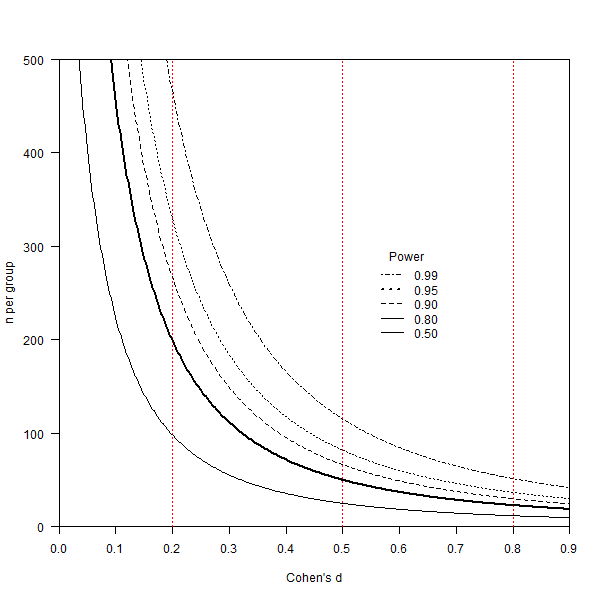
\includegraphics[height=.8\textwidth]{images/power}
\end{center}
}



\section{Practicalities}
\frame{\tableofcontents[currentsection]}

\frame{\frametitle{Some final considerations}
\begin{enumerate}
\item Ethics
\item Compliance
\item Effect Moderation
\item Mediation/mechanisms
\end{enumerate}

}


\frame{
\frametitle{Ethics}
\begin{itemize}
\item Experiments raise lots of ethical considerations
\item Because we are intervening in peoples' lives, we have to weight harm and benefits of our interventions
\item A big question relates to ``deception'' (are we deceiving our experimental participants? is that a problem?)
\end{itemize}
}


\frame{
\frametitle{Compliance I}
\begin{itemize}
\item Compliance is when individuals receive and accept the treatment to which they are assigned
\item Non-compliance is when participants receive the wrong treatment (cross-over) or simply fail to receive the treatment to which they are assigned
\item This causes problems for our analysis because factors other than randomization explain why individuals receive their treatment
\item Lots of methods for dealing with this, but the consequence is generally reduced power
\end{itemize}
}

\frame{
\frametitle{Asymmetric Noncompliance}
\begin{itemize}
\item If noncompliance only occurs in one group, it is \textit{asymmetric}
\item We can ignore non-compliance and analyze the ``intention to treat'' effect, which will underestimate our effects because some people were not treated as assigned\\
	$ITT = \overline{Y}_1 - \overline{Y}_0$
\item We can use ``instrumental variables'' to estimate the ``local average treatment effect'' (LATE) for those that complied with treatment:\\
	$LATE = \frac{ITT}{Percent Compliant}$
\item We can ignore randomization and analyze data ``as-treated'', but this makes our study no longer an experiment
\end{itemize}
}

\frame{
\frametitle{Two-Sided Noncompliance}
\begin{itemize}
\item Two-sided noncompliance is more complex analytically
\item Stronger assumptions are required to analyze it and we won't discus them here
\item Best to try to develop a better design to avoid this rather than try to deal with the complexities of analyzing a broken design
\end{itemize}
}


\frame{
\frametitle{Effect Moderation}
\begin{itemize}
\item Sometimes effect might vary across individuals or contexts
\item This is called \textit{moderation} or \textit{effect heterogeneity}
\item If we suspect this happens, we should design a complex experiment in which we manipulate the moderator
\item This way we can estimate ``conditional average treatment effects'' (CATEs) for each subgroup
\end{itemize}
}

\frame{
\frametitle{Effect Mediation}
\begin{itemize}
\item Sometimes we care about \textit{why} an effect comes about (i.e., what is the mechanism?)
\item This is called \textit{mediation}
\item If we suspect this happens and we care about the mediation process, we should try to manipulate the treatment and the suspected mediator
\item If we cannot manipulate the mediator, there is basically no credible way of estimating the ``mediation effect'' of the treatment group a given mediator
\end{itemize}
}



\appendix
\frame{}

\end{document}
